\chapter{Data distribution and visualization}
\label{chap:display}

This chapter focuses on user interface and \ac{API} provided by the project. In first section, \ac{API} is described. It serves both user interface and allows integration of external services. The next section covers user interface, graphs and features available to the end user. Python framework Flask requires route declaration so all routes concerning \ac{HTTP} communication are declared in a separate file. File is separated in 3 parts - first part exposes routes to web pages, next part serves \ac{API} functionality while the third part serves data for the graphs.


\section{Application programming interface}

Implemented \ac{API} provides data for both external services and for internal requirements. \ac{URL} for \ac{API} routes is distinguished by \code{/api}. Data served by \ac{API} is in \ac{JSON} format and is structured to be both human and machine readable. Accessing \code{/api/system} provides the list of all of the nodes with their names, \ac{id}s, timestamps of latest update and with list of attached sensor \ac{id}s. This allows external services to navigate though the system and query specific nodes and sensors for values. \code{/api/node} accepts node \ac{id} as a parameter and serves node id, name, list of attached sensor ids and last update timestamp. An example \ac{URL} for accessing node with id 1 would be \code{/api/node?id=1}. When sensor is accessed using \code{/api/sensor?id=1}, last update, last value, parent node id and sensor position on that node are displayed. If external service wants to access value history for a specific sensor this can be done via route \code{/api/sensor{\_}value} with supplied sensor id as a parameter. If no other parameter is received, server will provide array with 50 latest readings. Result is structured in such a way that it timestamp is a key for value at that given time. On that same route simple filtering can be introduced using start and end timestamps. By default, 50 latest readings are provided but more or less can be accessed using \code{readings} as a parameter. An example of data provided by accessing api route with start, end and number of readings parameters is seen in Listing \ref{lst:api_filter} while an overview of all of the model routes can be found in Table \ref{tab:web_api_model}.\\

\begin{lstlisting}[language=json,firstnumber=1,caption={API result for first 5 readings done in a set period of time},label={lst:api_filter}]
  {
    "result": {
      "2017-08-19-19-28-47": 17181, 
      "2017-08-19-19-28-50": 8522, 
      "2017-08-19-19-28-53": 1275, 
      "2017-08-19-19-28-57": 41146, 
      "2017-08-19-19-29-00": 45302
    }
  }
\end{lstlisting}

\begin{table}[h]
  \begin{center}
    \begin{tabular}[h]{ | >{\arraybackslash} p{3.5cm} | >{\arraybackslash} p{3cm} | > {\arraybackslash} p{7cm} |  }
      \hline
      Route & Parameters & Description \\ 
      \hhline{|=|=|=|}
      /api/node & id & Returns the timestamp of last node update, it's name and list of all available sensors \\[1ex]
      /api/sensor & id & Returns the position of the sensor, last value and its timestamp \\[1ex]
      /api/sensor{\_}value & id, readings, start, stop & By default returns last 50 values read by the sensor specified by the supplied id. Time period of readings can be filtered by start and stop timestamps. Readings parameter filters the number of readings. \\
      \hline
    \end{tabular}
  \end{center}
  \caption{System model description API routes.}
  \label{tab:web_api_model}
\end{table}

The next part of the \ac{API} concerns the charts. Most of the charts are implemented using \href{http://www.chartjs.org}{Chart.js} javascript library while \href{https://plot.ly}{plotly} is used for heath map. All of the charts are updated in real time but can also show history so \ac{API} was designed to support these features. The first chart user is greeted with is histogram of all sensor values. This graph helps live setup of the sensors. Users can easily indicate issues with connection or positioning of the sensors. The next graph is node graph - for each sensor attached to the selected node it shows the history how the values changed through time. It's also possible to view a single node history graph. The last graph is heath map of the bed which shows the topological preview of the sensor grid. With the increase of weight detected by the sensor, fields become red while with the decrease they become blue. \ac{API} allows user interface to specify the time for which sensor data should be shown. Graph data can be accessed using path \code{/api/chart} and is also served in \ac{JSON} format. Systematical overview of all chart routes is found in Table \ref{tab:web_api_charts}.

\begin{table}[h]
  \begin{center}
    \begin{tabular}[h]{ | >{\arraybackslash} p{3.5cm} | >{\arraybackslash} p{3cm} | > {\arraybackslash} p{7cm} |  }
      \hline
      Route & Parameters & Description \\ 
      \hhline{|=|=|=|}
      /api/chart/heatmap &  & Returns 0xab (1B) \\[1ex]
      /api/chart/histogram &  & Returns 0xab (1B) \\[1ex]
      /api/chart/node &  & Returns 0xab (1B) \\[1ex]
      /api/system &  & Returns the system overview with node and sensor ids \\ 
      \hline
    \end{tabular}
  \end{center}
  \caption{API routes used providing the chart data.}
  \label{tab:web_api_charts}
\end{table}

It's also possible to see the status of the data acquisition service using path \code{/api/service}. This route will return true if the service is running and false if service is inactive. It's also possible to start and stop service accessing start or stop \ac{API} routes. These routes will execute the procedure for either starting or stopping the service and then return if the action was successful. To redistribute addresses to I2C nodes, a route \code{/api/distribute} is used. Accessing it will execute the redistribution routine. Since user might want to save different sleep sessions it's also possible to save the start or end of the active session using route \code{/api/session}. All of these routes can be used by external services but are also used by web user interface. To avoid the whole page reloading for every new chart update, \ac{AJAX} technique was used but with \ac{JSON} replacing \ac{XML}. A list of all \ac{API} routes with their descriptions can be seen in Table \ref{tab:web_api_system}. Routes are serving GET requests but it's easily possible to transfer them to POST requests in which user session info or external token info would be saved. This would protect the data from unauthorized access but this is not needed for this stage of the project.

\begin{table}[h]
  \begin{center}
    \begin{tabular}[h]{ | >{\arraybackslash} p{3.5cm} | >{\arraybackslash} p{3cm} | > {\arraybackslash} p{7cm} |  }
      \hline
      Route & Parameters & Description \\
      \hhline{|=|=|=|}
      /api/distribute &  & Redistributes the node addresses based on their physical position \\[1ex]
      /api/service &  & Returns if the data acquisition service is running \\
      /api/service/start &  & Starts the data acquisition service, returns the operation outcome \\[1ex]
      /api/service/stop &  & Stops the data acquisition service, returns the operation outcome \\[1ex]
      /api/session &  & Returns if session is in progress and its id \\
      /api/session/start &  & Starts a new session if another session is not active \\[1ex]
      /api/session/stop &  & Stops the session if there is an active session in progress \\
      \hline
    \end{tabular}
  \end{center}
  \caption{API routes for controlling the system with described functions.}
  \label{tab:web_api_system}
\end{table}

\section{User interface}

Python Flask framework follows \ac{MVC} rules regarding the separation of logic. Model and a part of controller were already presented but this section will focus mainly on view and its integration. Flask uses \href{http://jinja.pocoo.org/docs/2.9/}{Jinja2} template engine which allows specific web pages to easily implement and extend template design. It also allows injection of data and control logic into the view. This means that data objects can be passed directly from the controller while control logic like loops or if clauses may be used to construct the page that will in the end be rendered. For each of the pages a separate template is created in \code{app/templates/} folder. \code{base.html} is a template which all other pages extending. It implements \ac{HTML} headers, user interface parts such as sidebar, header and footer. It links all of \ac{CSS}, javascript pages and allows insertion of page specific javascript files in separate block. File \code{/app/views.py} holds the request routing logic. Based on the received \ac{HTTP} requests, program renders different templates by inserting required data objects. A bigger part of user interface design is based on \href{coreui.io}{CoreUI} \href{http://getbootstrap.com/}{Bootstrap} admin interface template. The template was modified and structured to work as a Jinja2 template. CoreUI is licensed under MIT license\cite{coreui-license} and can be used and distributed free but with the preservation of license.

As it was already mentioned, website was designed to allow live updating and graphics rich design. For that, multiple javascript libraries were used. Some of them are jQuery, Bootstrap, chart.js and plotly. To take care of these dependencies, bower was used. On \ac{CSS} side, Bootstrap was extended by a custom script.

So how do these template generated, javascript and css infused pages look and what do they do? First thing a user is greeted with is a dashboard. It shows the number of currently present nodes and sensors and state of the data acquisition service. It also shows the histogram which helps the user see if system is working properly. In a case when there is no pressure on the bed, all of the sensors should be at the left of the chart where 0 is located. When person lies on the bed, the chart changes and values get redistributed throughout the chart. The dashboard can be seen in Figure \ref{fig:interface_histogram}.

\begin{figure}[h]
  \begin{center}
    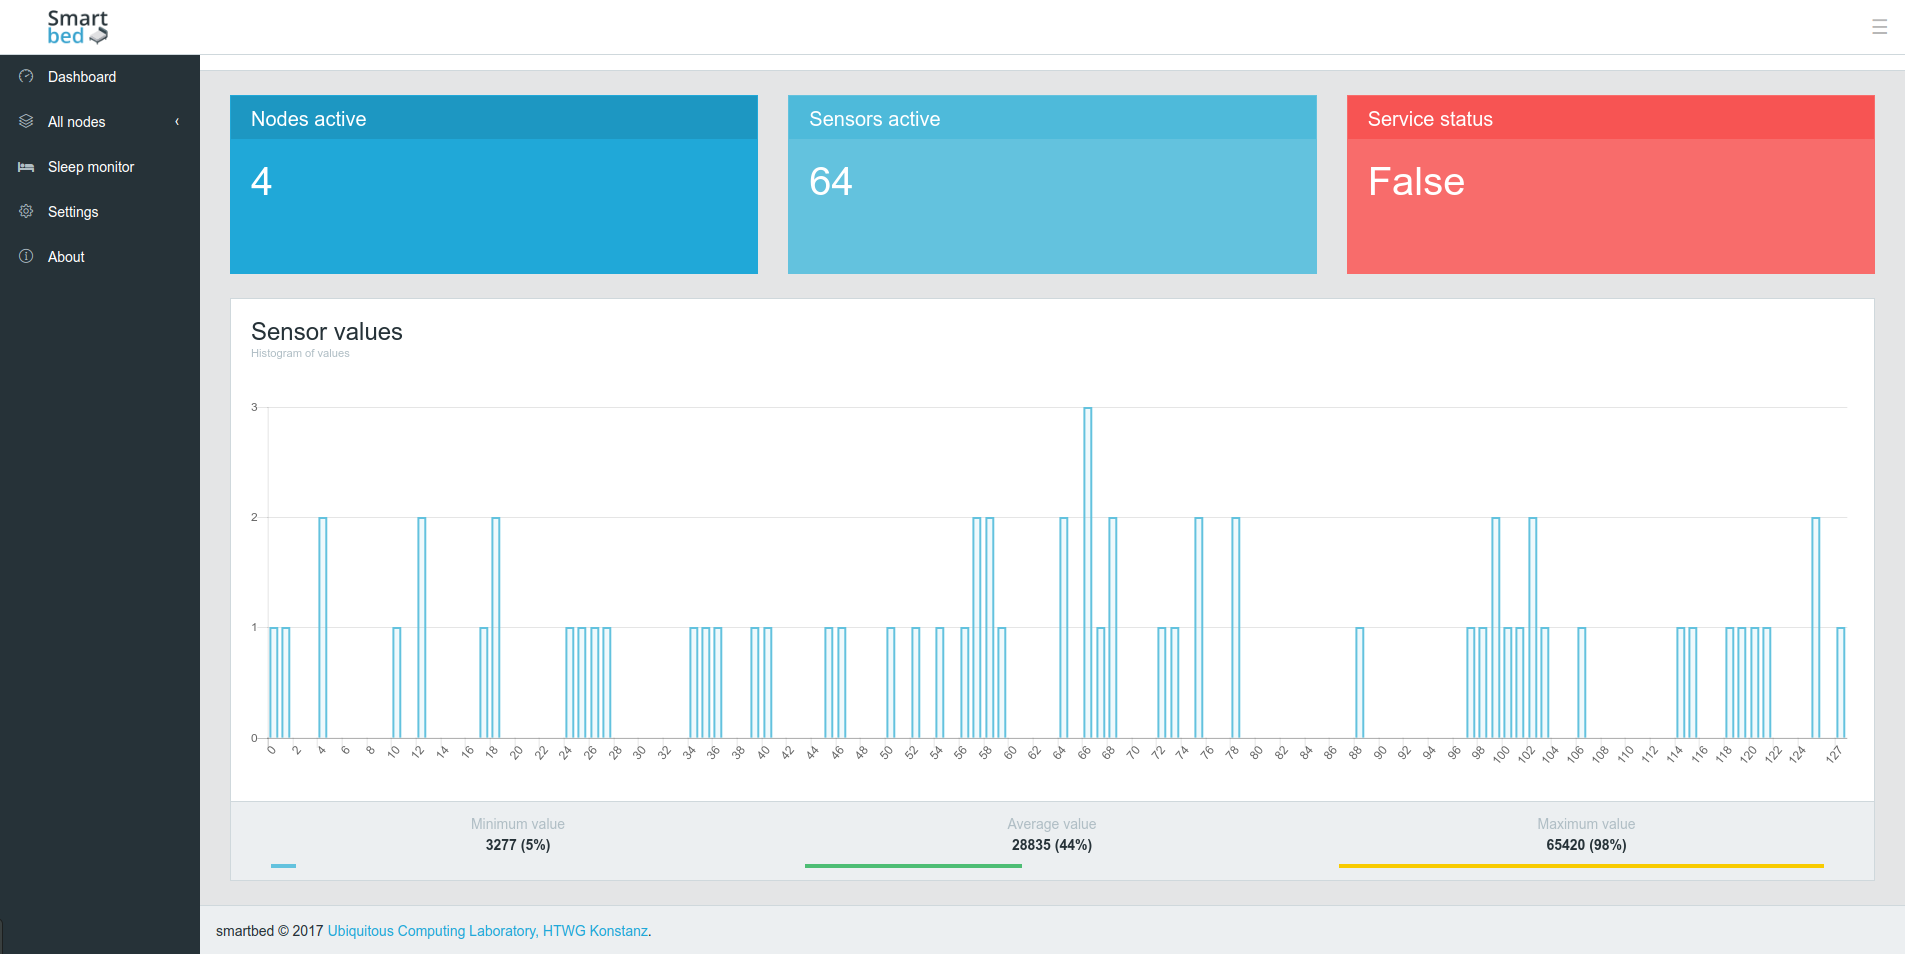
\includegraphics[width=\linewidth]{4-interface_histogram.png}
  \end{center}
  \caption{Flow diagram of data acquisition process.}
  \label{fig:interface_histogram}
\end{figure}

To observe the nodes and adjust the values, node view displays line charts of all attached sensor values. Graphs are updated periodically and latest value is displayed in the appropriate card. If sensor needs to be adjusted, this can be done though modal window for scaling and offsetting. For example, if the weight of the pillow or some other object is affecting the zero-weight reading, it's possible to offset the future sensors readings. Described view is shown in Figure \ref{fig:interface_sensors}.

\begin{figure}[h]
  \begin{center}
    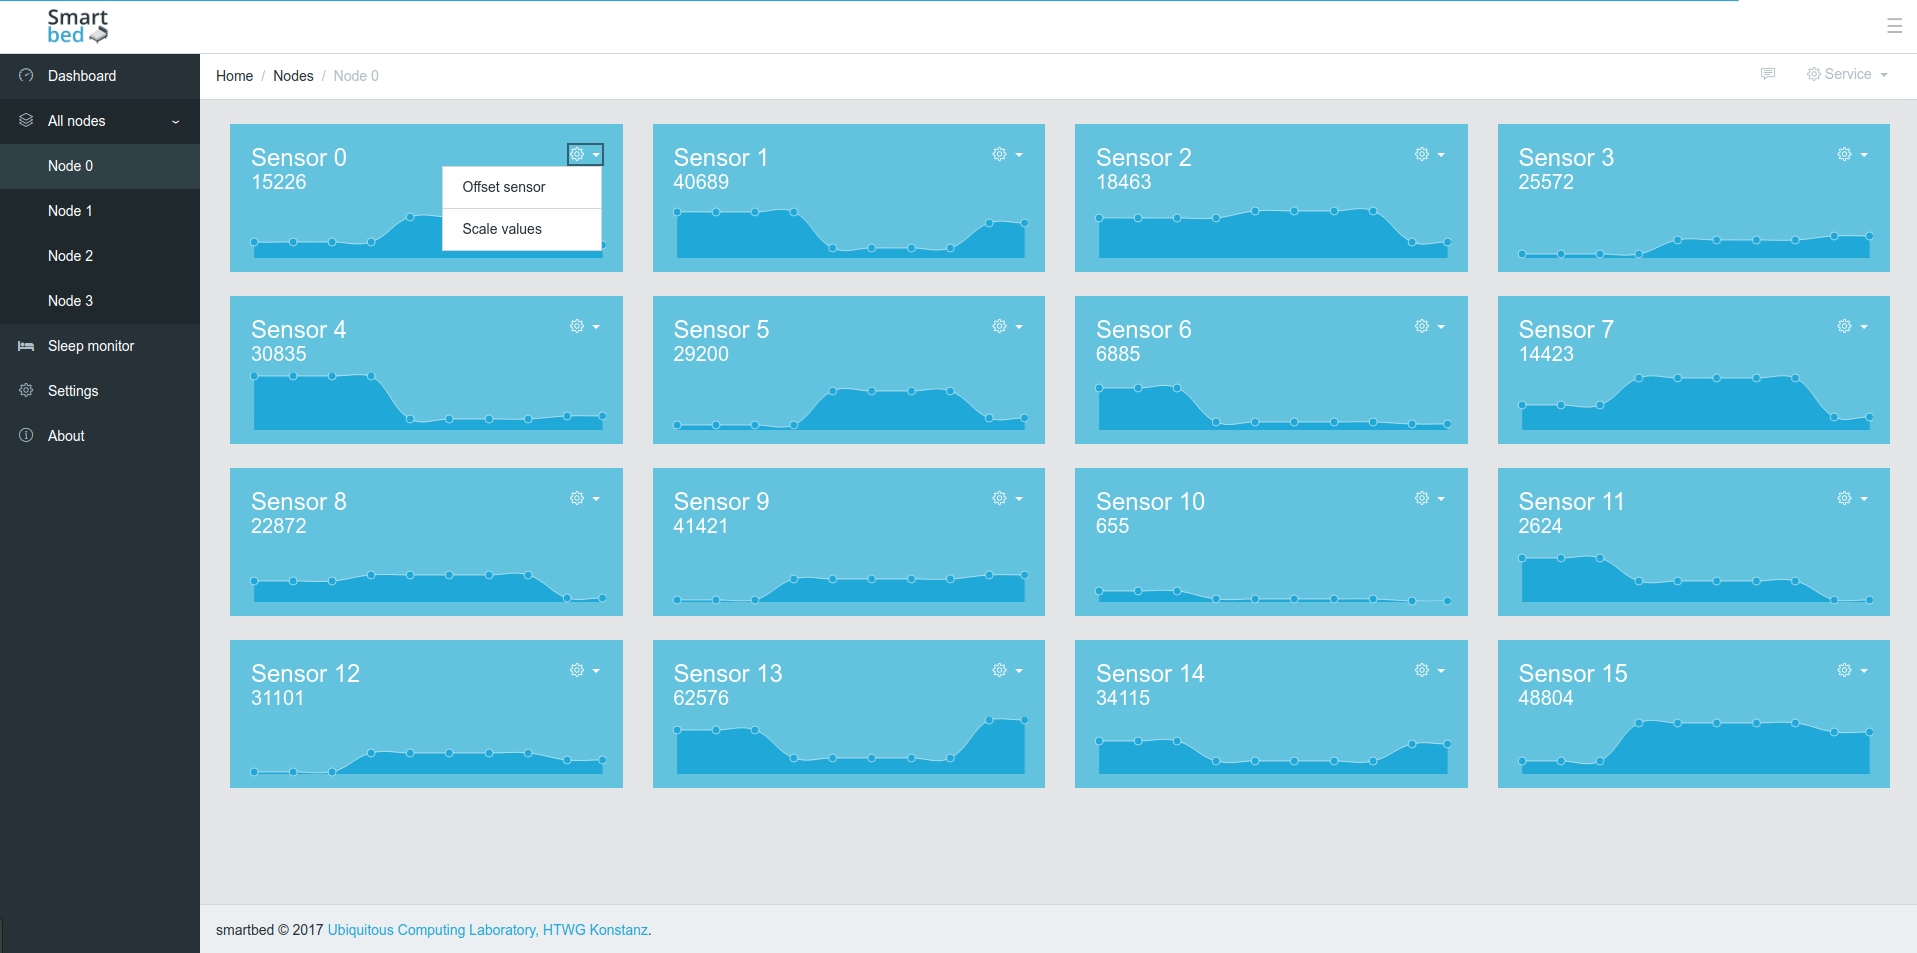
\includegraphics[width=\linewidth]{4-interface_sensors.png}
  \end{center}
  \caption{Flow diagram of data acquisition process.}
  \label{fig:interface_sensors}
\end{figure}

To help future research which will focus on sleep position recognition, a heat map was implemented. It shows the topological view of the bed with all of the attached sensors. Each sensor is represented by a colored rectangle which changes it's color depending on the pressure applied to it. There is also a possibility to view previous values so a pose of person sleeping in the bed can be observed through the night. This chart is presented in Figure \ref{fig:interface_heatmap}.

\begin{figure}[h]
  \begin{center}
    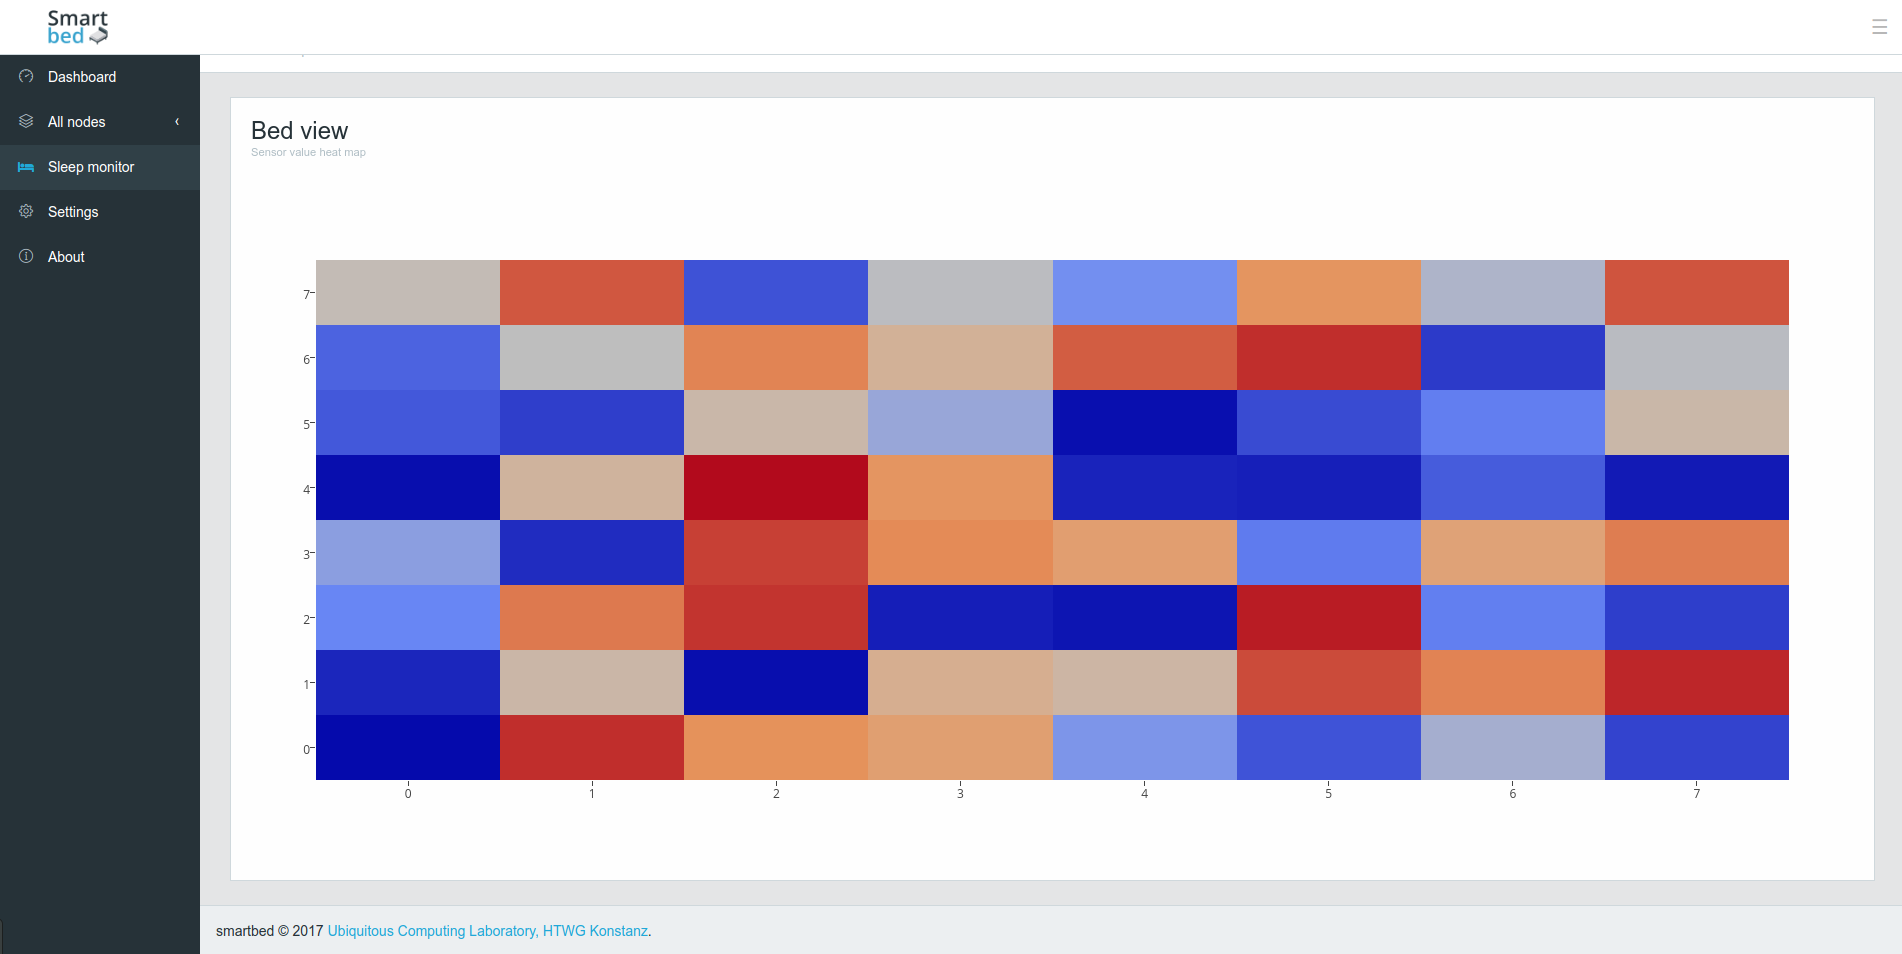
\includegraphics[width=\linewidth]{4-interface_heatmap.png}
  \end{center}
  \caption{Flow diagram of data acquisition process.}
  \label{fig:interface_heatmap}
\end{figure}

The whole interface was also adapted to work with the mobile devices. In case of the lower resolutions, page elements are redistributed and resized to fit the smaller screen. Navigation transfers to the 'hamburger' menu implemented sidebar while the rest of the functionality remains unchanged.

\begin{figure}[h]
  \begin{center}
    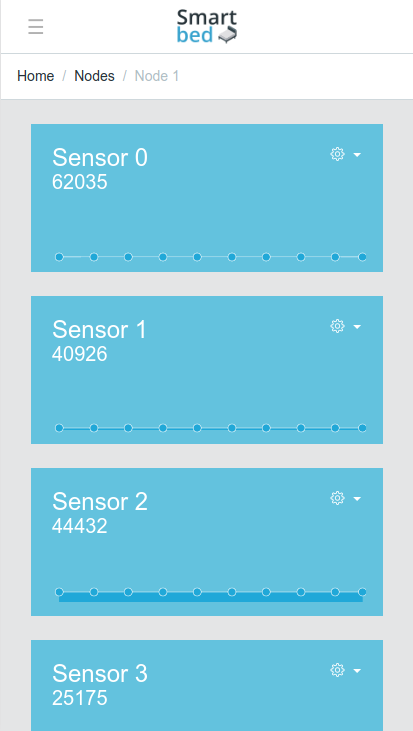
\includegraphics[width=0.3\linewidth]{4-interface_mobile.png}
  \end{center}
  \caption{Flow diagram of data acquisition process.}
  \label{fig:interface_mobile}
\end{figure}